\documentclass[11pt,a4wide]{article}
\usepackage{verbatim}
\usepackage{listings}
\usepackage{graphicx}
\usepackage{a4wide}
\usepackage{color}
\usepackage[options]{SIunits}
\usepackage{amsmath}
\usepackage{amssymb}
\usepackage[dvips]{epsfig}
\usepackage[utf8]{inputenc}
\usepackage[OT1]{fontenc}
\usepackage{cite} % [2,3,4] --> [2--4]
\usepackage{shadow}
\usepackage{hyperref}

\setcounter{tocdepth}{2}
%
\lstset{language=c++}
\lstset{alsolanguage=[90]Fortran}
\lstset{basicstyle=\small}
\lstset{backgroundcolor=\color{white}}
\lstset{frame=single}
\lstset{stringstyle=\ttfamily}
\lstset{keywordstyle=\color{red}\bfseries}
\lstset{commentstyle=\itshape\color{blue}}
\lstset{showspaces=false}
\lstset{showstringspaces=false}
\lstset{showtabs=false}
\lstset{breaklines}

\begin{document}
\title{report on project solar system}
\author{Ekaterina Ilin and Isabelle Gauger\\GitHub: \url{https://github.com/CPekaterina/Solar-System}
}
\maketitle
\tableofcontents
\newpage
\section{Introduction}
In this report we present methods to simulate the Solar system using numerical methods to solve the $n$-body problem that is determined by Newton's second law.  Using the Verlet and the Runge Kutta 4 (RK4) algorithms we first solve the two-body problem including the Earth and the Sun in a fixed position, then the 3-body problem in which we add Jupiter and vary its mass. In contrast to the first the latter has no closed form solution any more. Finally we include all planets from the Solar system into the calculations.
\section{The equations of motion}
The movement of a body $j$ with the mass $m_A$ and the coordinate $\vec{r}$ in a system of $p$ bodies with masses $m_i$  and coordinates $\vec{r}_i$ at any given time is described by Newton's second law:
\begin{equation}
\dfrac{\mathrm d^2 \vec{r}_j}{\mathrm d t^2}=\displaystyle\sum_{k=0 \wedge i\neq j}^{p}\left(-\dfrac{G\cdot m_k}{\left|\vec{r}_j-\vec{r}_k\right|^2}\right)
\label{eq:Newton}
\end{equation}
Here $G$ is the gravitational constant.  For legibility we assume that $p=2$  and drop the index $j$ because as we will see the used methods stay the same for any number of bodies involved.This equation is a second order differential equation that we split up into a set of coupled first order differential equations:
\begin{equation}
\dfrac{\mathrm d\vec{v}}{\mathrm d t}=-\dfrac{G\cdot m_k}{\left|\vec{r}-\vec{r}_k\right|^2}=f(\vec{r},\vec{r}_k)\quad\wedge\quad \dfrac{\mathrm d\vec{r}}{\mathrm d t}=\vec{v}
\label{eq:cNewton}
\end{equation}
$\vec{v}$ is then the velocity of the body. 
\\
Two very popular methods for solving coupled first order differential equations are the Verlet and the Runge Kutta 4 algorithms which are explained in the next two chapters.
\subsection{The Verlet method}
The Verlet method allows us to solve these two first order differential equation by expanding the coordinates at a time $t_i$ for $t_{i+1}=t_i+h$ and $t_{i-1}=t_i-h$. For each coordinate $x^l$ with corresponding velocity $v^l$ and the acceleration
\begin{equation}
f^l(\vec{r},\vec{r}_k)=-\dfrac{G\cdot m_k\cdot (x^l-x_k^l)}{\left(\displaystyle\sum_l(x^l-x_k^l)^2\right)^{\frac{3}{2}}}
\label{eq:}
\end{equation}
for $l=1,2,3$ we obtain:
\begin{equation}
x_i^l(t_i+h)=x_i^l(t_{i+1})=x^l_{i+1}=x_i^l+h\cdot v_i^l+h^2/2\cdot f_i^l(\vec{r},\vec{r}_k)+O(h^3)
\label{eq:t1}
\end{equation}
\begin{equation}
x_i^l(t_i-h)=x_i^l(t_{i-1})=x^l_{i-1}=x_i^l-h\cdot v_i^l+h^2/2\cdot f_i^l(\vec{r},\vec{r}_k)+O(h^3)
\label{eq:t2}
\end{equation}
Adding up \ref{eq:t1} and \ref{eq:t2} yields:
\begin{equation}
x^l_{i+1}=2x_i^l-x_{i-1}+h^2\cdot f_i^l(\vec{r},\vec{r}_k)+O(h^4)
\label{eq:t}
\end{equation}
All odd powers of $h$ cancel out and we obtain a precision for each step that goes with $O(h^4)$. Given the initial conditions for $x^l_0$ we can compute $x^l_1$ using the initial velocity and then continue computing all following time steps:
\begin{equation}
x^l_1=x^l_0+h\cdot v^l_0+\dfrac{h^2}{2}f_0^l
\label{eq:t0}
\end{equation}
If there are several bodies involved this procedure has to be performed for each time step for every body and thus move the system to the next time step. In this case $f_i^l$ is obtained via equation \ref{eq:Newton} that means adding up all gravitational forces that one of the bodies experiences to compute the resulting acceleration.
\\
The Verlet method does not give us any information about $\vec{v}_i$ but it can be easily derived from the positions $\vec{r}_{i+1}$ and $\vec{r}_{i-1}$:
\begin{equation}
v^l_i=\dfrac{x^l_{i+1}-x^l_{i-1}}{h}+O(h^2)
\label{eq:v}
\end{equation}
The overall error for the Verlet method is $O(h^3)$ for the positions and $O(h)$ for the velocities. The RK4 method is more precise as it shall be shown in the next chapter. 
 \subsection{The Runge Kutta 4 method}
Another powerful algorithm that allows us to solve coupled first order differential equations with a global truncation error that goes like $O(h^4)$ is the Runge Kutta of the 4th order method (RK4). Given the equation
\begin{equation}
\dfrac{\mathrm d y}{\mathrm dt}=f(y,t)
\label{eq:diff1}
\end{equation}
and integrating both sides from $t_i$ to the next time step $t_{i+1}=t_i+h$ we obtain
\begin{equation}
y_{i+1}-y_i=\displaystyle\int_{t_i}^{t_{i+1}}f(y,t)\mathrm dt
\label{eq:int1}
\end{equation}
We use Simpson's rule to approximate the integral  which leads to
\begin{equation}
y_{i+1}=y_i+\dfrac{h}{6}\left(f(y_i,t_i)+4\cdot f(y_{i+1/2},t_{i+1/2})+f(y_{i+1},t_{i+1})\right) +O(h^5)
\label{eq:simp}
\end{equation}
Furthermore we split the intermediate step in to equal parts:
\begin{equation}
y_{i+1}=y_i+\dfrac{h}{6}\left(f(y_i,t_i)+2\cdot f(y_{i+1/2},t_{i+1/2})+2\cdot f(y_{i+1/2},t_{i+1/2})+f(y_{i+1},t_{i+1})\right) +O(h^5)
\label{eq:simp}
\end{equation}
Now we can estimate the values of $y$ inbetween $t_i$ and $t_{i+1}$ four times to get greater precision for the corresponding slopes.  We set
	\begin{eqnarray}
	k_1&=&h\cdot f(y_i,t_i)\\
	\label{eq:RKk1}
	k_2&=&h\cdot f(y_i+k_1/2,t_i+h/2)\\
	k_3&=&h\cdot f(y_i+k_2/2,t_i+h/2)\\
	k_4&=&h\cdot f(y_i+k_3,t_i+h)
	\label{eq:RKk}
	\end{eqnarray}
	$k_1$ obviously equals the first term in the brackets of \ref{eq:simp}. $k_2$ and $k_3$ are then used to approximate the second and third term and $k_4$ for the last one. If we include \ref{eq:RKk1} to \ref{eq:RKk}, equation \ref{eq:simp} is composed of the following terms:
\begin{equation}
y_{i+1}=\dfrac{1}{6}\left(y_i+h\cdot k_1\right) +\dfrac{1}{3}\left(y_i+h\cdot k_2\right)+\dfrac{1}{3}\left(y_i+h\cdot k_3\right)+\dfrac{1}{6}\left(y_i+h\cdot k_4\right) +O(h^5)
\label{eq:simpk}
\end{equation}
	Thus we compute the slopes at $y_i$ and $y_{i+1}$ once each and $y_{i+1/2}$ twice using the previous $k$-values in every step and end up with a local truncation error of  the order of $O(h^5)$ which leads to a global error that goes like $O(h^4)$.
	\\
	We apply RK4 to a set of coupled first order differential equations of the form
	\begin{equation}
  \dfrac{\mathrm d v}{\mathrm dt}=f(x,t) \quad\wedge\quad \dfrac{\mathrm d x}{\mathrm dt}=v
	\label{eq:New}
	\end{equation}
	To obtain $v_{i+1}$ and $x_{i+1}$ the algorithm's steps have to be performed in the following order:
	\begin{enumerate}
		\item $k_{1,x}=h\cdot v_i$ and $k_{1,v}$ are computed separately.
		\item $k_{2,v}$ is then computed as described above. 
		\item $k_{2,x}$ is derived from $k_{1,v}$ then: $k_{2,x}=h\cdot(v_i+k_{1,v}/2)$
		\item $k_{3,x}$ and $k_{3,v}$ are obtained as in steps 2. and 3. with $k_{3,x}=h\cdot(v_i+k_{2,v}/2)$
		\item $k_{4,x}$ and $k_{4,v}$ are computed as in 2. and 3. as well with $k_{4,x}=h\cdot(v_i+k_{3,v})$
	\end{enumerate}
	From here the values for $v_{i+1}$ and $x_{i+1}$ can be obtained from the formula \ref{eq:simpk} and the algorithm can be applied to the next time step.
	\\
	In the following chapters both algorithms are used to simulate the motion of the bodies in the solar system. It is convenient to implement the algorithms in an object oriented way. We decided for a class of planets. Its objects contain the main parameters of the bodies inside the solar system such as the mass and arrays of vectors for the position and velocities as well as the initial positions and velocities and some physical constants like $G$.
	\\
	The class also contain the functions \textbf{RK4}, \textbf{Verlet}, \textbf{RK4step} and \textbf{force} as well as some functions to write the results into data files. These functions perform the following tasks:
	\begin{description}
	\item[RK4] receives an array of the classes' objects and performs \textbf{RK4step} for a given number of time steps $n$ of certain step length $h$ and the number of objects $p$ which is also the size of the array. Then the velocities and positions for the next time step are computed for all planets before moving on to the next time step.
	\item[Verlet] receives the same data as \textbf{RK4} but performs the method directly inside the function and also computes the velocities.
	\item[RK4step] uses the values for the current time step and planet to compute the velocity and position for next time step for said planet. Here the RK4 algorithm is applied and the function \textbf{force} is used.
	\item[force] computes the gravitational force a certain planet experiences given the current positions and masses of all the other planets involved. 
	\end{description}
	\section{Earth-Sun system}
	In order to analyse the basic properties of both the Verlet and the RK4 methods we fix the Sun to the center of the coordinate system and only add Earth. This problem has a closed form solution. We want to discuss the case of a circular orbit and check the stability of the algorithms by comparing our results to the analytical solution. We are also going to check on the conservation of energy and momentum and find the escape velocity of Earth.
	\subsection{Circular orbit and stability}
	\begin{table}
	\centering%
	\caption{Stability of \textbf{Verlet} and \textbf{RK4}. $\Delta r$ is the distance of the position after 100\,yr to the initial position. $R$ is the approximated total distance over 100 yr ($R\approx 100\cdot 2\pi \,\text{AU}$).}
	\begin{tabular}{l|cr|cr}\hline
	$h$ in yr & \multicolumn{2}{c|}{ \textbf{Verlet} } & \multicolumn{2}{c}{\textbf{RK4}}\\\hline
	& $\Delta r$ in AU & $\Delta r/R$ in $\%$ & $\Delta r$ in AU & $\Delta r/R$ in $\%$ \\\hline
	$10^{-1}$ & $2.1$											& $3.3\cdot10^{-1}$ &  unstable     						& unstable                \\
	$10^{-2}$ & $0.9$											& $1.4\cdot10^{-1}$ &	 $5.5\cdot10^{-2}$ & $8.7\cdot10^{-3}$ \\
	$10^{-3}$ & $1.5\cdot10^{-2}$	& $2.3\cdot10^{-3}$ &  $6.3\cdot10^{-3}$ & $1.0\cdot10^{-3}$ \\
	$10^{-4}$ & $7\cdot10^{-4}$		& $1.1\cdot10^{-4}$ &  $6.3\cdot10^{-4}$ & $1.0\cdot10^{-4}$ 
	\end{tabular}
	\label{tab:stab}
	\end{table}
	
	\begin{figure}
		\centering
			\includegraphics[scale=0.45]{earth.pdf}
		\caption{The Earth orbits the Sun in the two-dimensional equatorial plane. The step length is $h=10^{-4}$ and $\Delta t=1$\,yr}
		\label{fig:earth}
	\end{figure}
	
	In the following considerations we introduce some convenient units: $1\,\text{AU}$ for distances, $1\,\text{yr}$ for time and $1\,\text{m}_{\text{S}}$ (Solar mass) for masses. The mass of the Earth is then $m_E=3\cdot 10^{-6}\,\text{m}__{\text{S}}$. The gravitational constant becomes approximately $G=4\pi^2\dfrac{\text{AU}^3}{\text{yr}^2\cdot \text{m}_\text{S}}$ in these units.
	\\
	For circular motion the centrifugal force is equal to the gravitational force:
	\begin{equation}
	\dfrac{m_E\cdot v^2}{r}=\dfrac{G\cdot m_S\cdot m_E}{r^2}
	\label{eq:cm}
	\end{equation}
	Assuming that the Earth is found at $r_0=1\,\text{AU}$ we find that the initial velocity has to be $v_0=2\pi\frac{\text{AU}}{\text{yr}}$ so that the Earth circles the Sun in exactly one year. Using these initial conditions we compute the motion of Earth around the fixed Sun for different step lengths expecting the circular motion to be stable. We use $\Delta t=100\,\text{yr}$ and use the distance from the last position of Earth to its initial one as a criterion for the stability. The results are shown in table \ref{tab:stab}. From this it can be concluded that the algorithm is quite stable for step lengths below $h=10^{-2}\,\text{yr}$ for \textbf{RK4} and below $h=10^{-3}\,\text{yr}$ for \textbf{Verlet}.
	\\
	In figure \ref{fig:earth} one can see the Earth's circular orbit around the Sun which is positioned in the center of the coordinate system. 
\subsection{Conservation of energy and momentum}

	\begin{figure}
		\centering
			\includegraphics[scale=0.45]{kinenergV.pdf}
		\caption{The kinetic energy of the Earth as it orbits the fixed Sun as computed with the \textbf{Verlet} method. The step length is $h=10^{-3}$ and $\Delta t=10$\,yr}
		\label{fig:ekv}
	\end{figure}
	
	\begin{figure}
		\centering
			\includegraphics[scale=0.45]{potenergV.pdf}
		\caption{The potential energy of the Earth as it orbits the fixed Sun as computed with the \textbf{Verlet} method. The step length is $h=10^{-3}$ and $\Delta t=10$\,yr}
		\label{fig:epv}
	\end{figure}
	
	
	\begin{figure}
		\centering
			\includegraphics[scale=0.45]{kinenergRK.pdf}
		\caption{The kinetic energy of the Earth as it orbits the fixed Sun as computed with the \textbf{RK4} method. The step length is $h=10^{-4}$ and $\Delta t=10$\,yr}
		\label{fig:ekrk}
	\end{figure}
	
	\begin{figure}
		\centering
			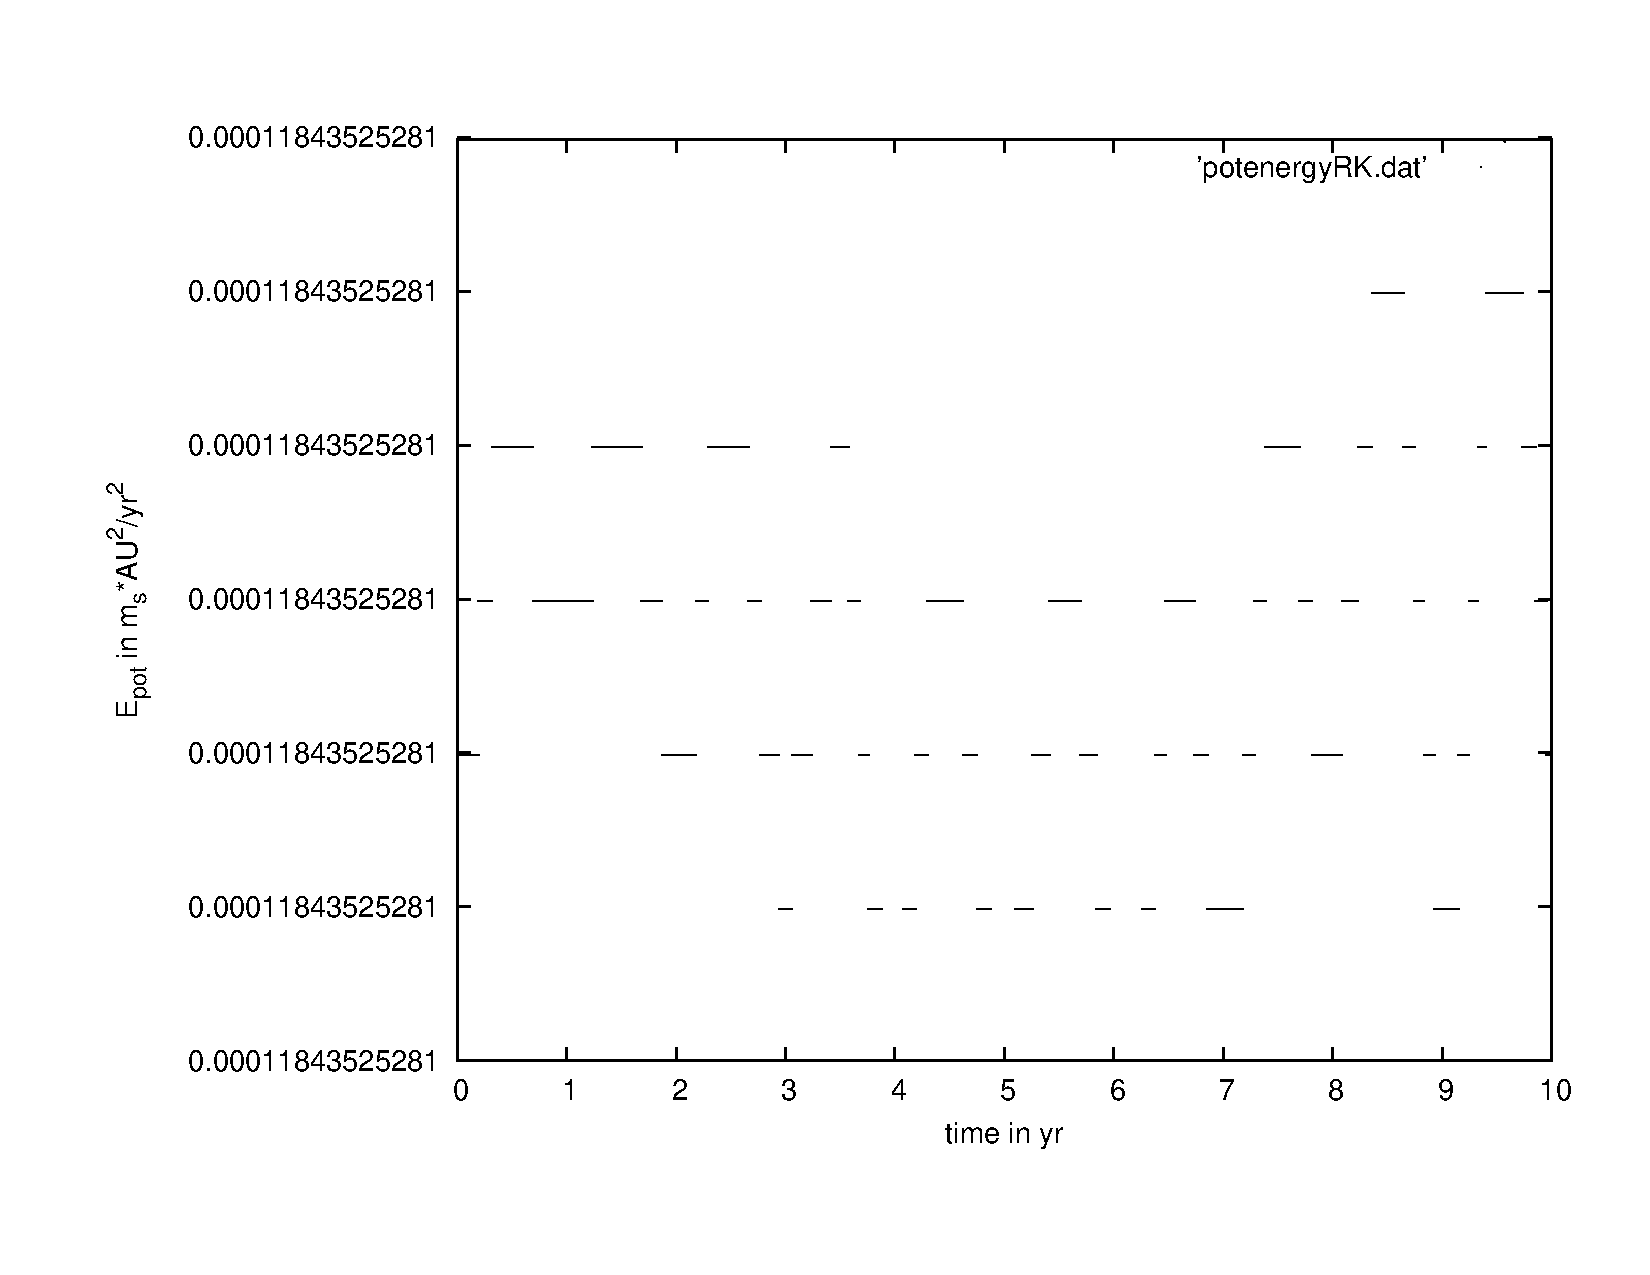
\includegraphics[scale=0.45]{potenergRK.pdf}
		\caption{The potential energy of the Earth as it orbits the fixed Sun as computed with the \textbf{RK4} method. The step length is $h=10^{-4}$ and $\Delta t=10$\,yr}
		\label{fig:eprk}
	\end{figure}
	
	\begin{figure}
		\centering
			\includegraphics[scale=0.45]{angmomV.pdf}
		\caption{The angular momentum of the Earth as it orbits the fixed Sun as computed with the \textbf{Verlet} method. The step length is $h=10^{-4}$ and $\Delta t=10$\,yr}
		\label{fig:amv}
	\end{figure}
	
	\begin{figure}
		\centering
			\includegraphics[scale=0.45]{angmomRK.pdf}
		\caption{The angular momentum of the Earth as it orbits the fixed Sun as computed with the \textbf{RK4} method. The step length is $h=10^{-4}$ and $\Delta t=10$\,yr}
		\label{fig:amrk}
	\end{figure}
We also check if the potential and kinetic energies $E_{pot}$ and $E_{kin}$ are conserved over time as well as the angular momentum $L_z$ as we only considered a movement in the equatorial plane for testing purposes. These values have to be conserved for the following reasons:
 \begin{description}
	\item[kinetic energy] This has to be conserved because the velocity of a body that is moving on a circular orbit is not supposed to change since the force is always perpendicular to the direction of the velocity.
	\item[potential energy] The potential energy in a gravitational field of a mass point is determined by the distance to this mass point. Because this is given on a circular orbit the potential energy stays constant.
	\item[angular momentum] Since the Earth-Sun system is a closed system and the angular momentum of the Sun is zero and does not change since it is fixed the angular momentum of the Earth has to constant as well.
 \end{description}

The figures \ref{fig:ekv}-\ref{fig:amrk} show the behaviour of the energies and the angular momentum for both \textbf{RK4} and \textbf{Verlet}. For the Verlet algorithm being a symplectic integrator (see \cite{Donnelly}) we find the kinetic and potential energies to be constant over the period of one year but fluctuating in a small range in between. The RK4 method does not show any significant fluctuations of kinetic or potential energies for step lengths of $h=10^{-4}$ and below although this error increases over long periods of time($>100$\,yr). 
\\
The angular momentum, however, is fairly constant for both methods as figures \ref{fig:amv} and \ref{fig:amrk} show.  
\subsection{Escape velocity of the Earth}
We now consider a planet that has the same distance from the sun than earth and want to find out what initial velocity it at least must have to escape from the sun. By trial and error we find an escape velocity of $8.9\frac{\text{AU}}{\text{yr}}$ what is $42332.6\frac{\text{m}}{\text{S}}$. At the starting time $t1$ our planet has the velocity $v$ and the distance $r$ from the sun. So it's total energy is given by

\begin{equation}
E_{total}\left(t_1\right) = E_{kin}\left(t_1\right) + E_{pot}\left(t_1\right) = \frac{1}{2}m_{p}v^2 - \frac{Gm_{S}m_{p}}{r}
\end{equation}

We choose $t_2$ as a later point in time when our planet is far away from the sun. The total energy of our planet is then

\begin{equation}
E_{total}\left(t_2\right) = E_{kin}\left(t_2\right) + E_{pot}\left(t_2\right) 
\end{equation}

For $r\rightarrow\infty$ the potential energy of our planet is zero. Our aim is to find the minimum velocity with which our planet escapes the Sun's gravitational field so we also set the kinetic energy to zero for $t_2$. The total energy has to be preserved what leads to

\begin{equation}
E_{kin}\left(t_1\right) + E_{pot}\left(t_1\right) = E_{kin}\left(t_2\right) + E_{pot}\left(t_2\right) = 0
\end{equation}

which is equal to 

\begin{equation}
\frac{1}{2}m_{p}v^2 - \frac{Gm_{S}m_{p}}{r} = 0
\end{equation}

We rearrange that and get the escape velocity

\begin{equation} 
v=\sqrt{\frac{2Gm_{S}}{r}}=\sqrt{\frac{2*6,67*10^{-11}\frac{\text{m}^3}{\text{kg}\text{s}^2}*2*10^{30}\text{kg}}{1,5*10^{11}\text{m}}}=42174.2\frac{\text{m}}{\text{s}}
\end{equation}

The value we obtain for the escape velocity by trial and error is around the exact solution but of course not very precise.  
\section{The entire solar system}
Finally we include the other planets Mercury (see \cite{wiki:1}), Venus (see \cite{wiki:2}), Mars(see \cite{wiki:4}), Saturn((see \cite{wiki:6}), Uranus (see \cite{wiki:7}), Neptun ((see \cite{wiki:8}) and also the dwarf planet Pluto (see \cite{wiki:9}). Their initial positions from the 1.10.14 are extracted from \cite{astro} and \cite{NASA}. The Suns's initial velocity is set to obtain a total momentum of zero and the time interval is 1200\,yr. The results for the inner (up to Mars) and outer Solar System are shown in figures \ref{fig:solsysin} and \ref{fig:solsysout}.
\\
One can clearly see that with the given inital velocities and positions the  trajectories of the planets and Pluto are stable for at least 1200\,yr. Furthermore, we observe a high eccentricity of Pluto. 
	\begin{figure}
		\centering
			\includegraphics[scale=0.55]{1200yr.pdf}
		\caption{The inner solar system. The step length is $h=10^{-3}$ and $\Delta t=1200$\,yr}
		\label{fig:solsysin}
	\end{figure}
	
	
	\begin{figure}
		\centering
			\includegraphics[scale=0.55]{1200yrout.pdf}
		\caption{The outer solar system. The step length is $h=10^{-3}$ and $\Delta t=1200$\,yr}
		\label{fig:solsysout}
	\end{figure}
\bibliographystyle{plain}
\bibliography{biblio}

\end{document}
 